\chapter{Introduction}
	%  - Introduction 
			%- 	CMB 
			%- 	Cosmological Parameters
\section{Modern Cosmology, and the Cosmic Microwave Background}
Modern cosmology has been experiencing a golden age since the 1990s. Access to larger and larger datasets has allowed astronomers to develop increasingly more detailed models of the universe. These models rely on several fundamental assumptions stemming from observation, the chief of which is the Big Bang Model. 
\par In 1929, Edwin Hubble confirmed a relation earlier found by Georges Lemaître, between  distances to galaxies and their recessional velocities: galaxies appear to be moving faster away from us, the further away they are \citep{1929PNAS...15..168H}. These observations gave rise to the Hubble Law,
\begin{equation}
	v  \varpropto d
	\label{eq:HubbleLaw}
\end{equation}
where $v$ is the velocity of a galaxy in question, and $d$ is its distance from us. 
\par To the best of our knowledge, there is nothing that suggests that our position in the universe is special or unique, a concept known as the Copernican Principle \citep{peacock_peacock_1998}. This leads to the logical extension that if every point in the universe is moving away from every other point, the universe must be expanding. If we reverse the flow of time, the universe must have been an incredibly hot, dense environment at some point in the past, a singularity known as the \emph{Big Bang}.
\par This singularity then expanded outwards, bringing into existence the early universe. Small fluctuations present in quantum fields, resulting from Heisenberg's Uncertainty Principle, created small inhomogeneities which seeded the universe with elementary quantum objects, such as quarks, gluons, photons, and dark matter. These particles swirled in a primordial fluid, mixing together, until eventually the universe cooled to a point that all the elements of the mixture stopped interacting with (i.e. de-couple from) each other. 
\par This early exponential expansion allowed the universe to mix, and so achieve a very high level of isotropy. Observationally, there appears to be no favoured direction in the universe, since distributions of distant galaxies and other extragalactic sources seem to be even across the sky. Perhaps the most spectacular example of this isotropy is the presence of the \emph{Cosmic Microwave Background} (CMB).
\par Discovered in 1964 \citep{Penzias:65} as a source of noise in another microwave experiment, over the next 30 years, it was noticed that there was isotropic black-body radiation everywhere in the universe, at a temperature of $T \approx \SI{2.7}{\kelvin}$. This radiation is most intense in the microwave section of the electromagnetic spectrum, it was named the cosmic microwave background.
\begin{figure}[ht]
	\centering
	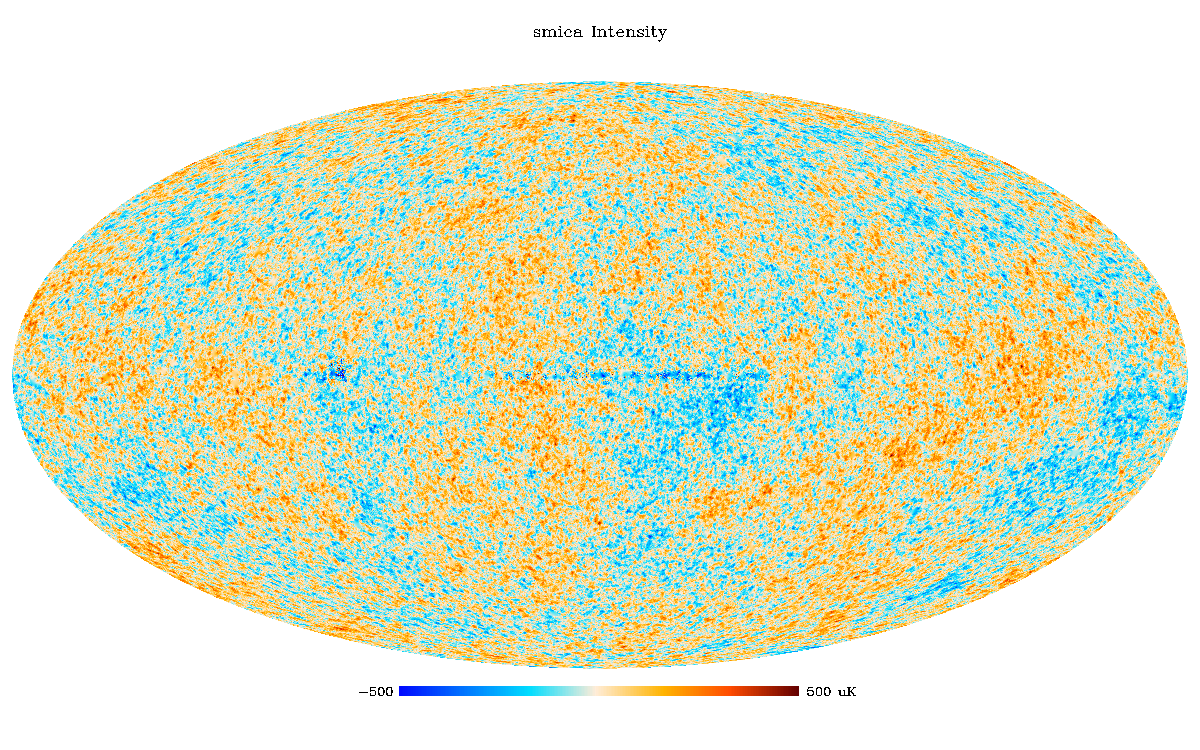
\includegraphics[scale=0.25]{/home/mitchell/Documents/masters/masters/thesis/Images/CMB_smica_tsig.png}
	\label{CMB Map}
	\caption{\emph{Planck} Satellite Full Sky CMB Map, extracted using the SMICA method \citep{2018arXiv180706205P}. This  map was produced by linearly combining the full spectrum of frequencies observed by the \emph{Planck} satellite from $\SI{30}{\giga\hertz}$ to $\SI{857}{\giga\hertz}$ in frequency space. Each map is first converted to its power spectrum, and then weighted at various multipoles, in order to account for contamination which appears at characteristic scales in different frequencies.}
\end{figure}

The CMB is a near-perfectly uniform field of background radiation which permeates the universe. Intially believed to be featureless, today the CMB is known to have very specific inhomogenaities, shown in \ref{CMB Map}. The uniformity of the CMB is the closest measurement we have to a perfect black-body, but with variations of approximately one part in 100,000, and an RMS of $\SI{18}{\micro\kelvin}$ \citep{2004mmu..symp..291W}. 

Theory holds that a very short time after the Big Bang ($\sim 10^{-37}$ seconds), the universe underwent an exponential growth period now termed \textit{inflation}. This phase is necessary to ensure that the universe is isotropic, flat, and gaussian, whilst also still taking into account the fact that opposite sides of the observable universe appear to be too far apart to ever have been causally connected. During this period, the universe was smoothed out, only leaving behind very small irregularities. These irregularities are what eventually gives rise to the large scale structure of the universe, what eventually would become the \emph{Cosmic Web}. 

As the universe adiabatically cooled, there was a considerable period of time, until approximately 380,000 years after the Big Bang, where photons were coupled to the other components of the universe, such as baryonic matter and dark matter. This period is what allowed for the quark-gluon plasma to mix appropriately, and develop waves in the fluid, ultimately resulting in the characterstic pattern in the CMB. This pattern is highly dependant on statistical parameters, and so the characterisitic angular size of the pattern of the CMB is incredibly sensitive to the relative proportions of the universe's matter-energy density. These charactersitic inhomogeneities can be decomposed into an angular power spectrum, which exibits a shape highly dependant on universal parameters. 

\begin{figure}[h!]
\centering
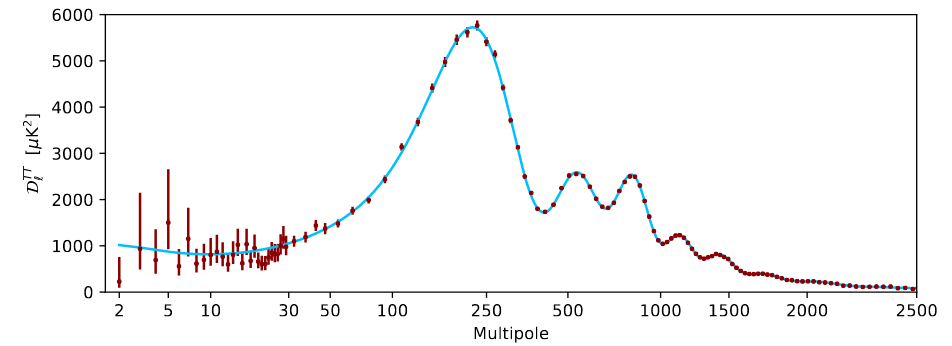
\includegraphics[scale=0.4]{/home/mitchell/Documents/masters/masters/thesis/Ver_2/figures/planck_2018.png}
\caption{\emph{Planck} 2018 Angular Power Spectrum \citep{2018arXiv180706209P}. The location, and relative heights of the first three peaks are sensitive to the overall energy density of the universe, as well as the relative amounts of baryonic matter and dark matter.}
\label{fig:power_spec}
\end{figure}

Shown in Figure \ref{fig:power_spec}, this angular power spectrum is very sensitive to cosmological paramters. Since the discovery of its anisotropy by \emph{Cosmic Background Explorer} (COBE) \citep{1992PhT....45f..17L}, and then its later refinement by \textit{Wilkinson Microwave Anisotropy Probe} (WMAP) \citep{2007ApJS..170..377S}, the power spectrum has been the gold standard by which astronomers measure cosmological parameters. The precision to which we know the CMB also makes it very good as constraining these parameters, leading many cosmologists to hold it as one of the most accurate measurements ever made in physics.  

\section{Cosmological Parameters}
The current accepted model, the $\Lambda$CDM model, contains six independant paramters which describe the evolution and behaviour of the universe: the physical baryon density $\Omega_b h^2$, the physical dark matter density $\Omega_c h^2$, the age of the universe $t_0$, the scalar spectral index $n_s$, the acoustic scale $100 \theta_\star$, and the reionisation optical depth $\tau$, the values of which are reported in Table \ref{table:params}. These primary parameters give rise to other parameters, such as the Hubble constant $H_0$ and its unitless form, known as the reduced Hubble constant $h$. It serves as a measure of the current rate of expansion of the universe, and carries units of $ \SI{}{\kilo\meter\per\second\per\mega\parsec}$. The Hubble constant is usually quoted for a number of reasons. Firstly, it contains both the age, and the size, of the universe within it, and secondly, it was one of the first cosmological parameters to be determined, back when Hubble was making his initial measurements, so it has some historical value. Because it is so ubiquitous, astronomers use different forms depending on what they are analysing, which becomes important for making direct comparisons between different measurements. When using the unitless form, if it lacks a subscript, it refers to the definition $h = H_0/\SI{100}{\kilo\meter\per\second\per\mega\parsec}$. Alternatively, if it carries one, it refers to replacing the number in the denominator with the number in the subscript, e.g. $h_{70} = H_0/\SI{70}{\kilo\meter\per\second\per\mega\parsec}$.

Currently, the highest precision measures of these features from the CMB come from the  \cite{2018arXiv180706209P} paper, which details that baryonic matter only comprises $\approx 5 \% $ of the universe's energy density. 

\par In principle, this component of the universe should be directly measurable. At just three minutes after the Big Bang, deuterium can be used as a tracer for this abundance \citep{2007ARNPS..57..463S}, and at a redshift $z \geqslant 2$, the baryon fraction can be found in the absorption lines of quasars passing through the diffuse, photo-ionised intergalactic medium, known as the Lyman-$\alpha$ forest \citep{1997ApJ...490..564W}. 

\par The baryon content has been confirmed very well at high redshift by the Planck collaboration, and the agreement between the CMB, and other independant high redshift measurements, such as baryon acousitc oscillations, and gravitational lensing reconstructions .  

\par However as the universe evolved, this gas became sparser, both as space expanded, and as it became more ionised by processes in the universe. This makes searching for the entirety of the baryon fraction at low redshift difficult, since high density objects are usually more easily detected. When this fraction is calculated for the local universe directly from observations, it shows only one tenth of the baryonic content shown in high redshift measurements is contained in galactic structures \citep{1992MNRAS.258P..14P}. This is troubling, because tensions in cosmological parameters between their high and low redshift measurments forces us to ask questions about the validity of cosmological models at all times.

\begin{table}[h!]
\centering
\begin{tabular}{||c c c||} 
 \hline
 Parameter & Value & Error \\
 \hline\hline
 $\Omega_c h^2$ & $0.120$ & $\pm 0.001$ \\
 \hline
 $\Omega_b h^2$ & $0.0224$ & $\pm 0.0001$ \\
 \hline
  $n_s$ & $0.965$ & $\pm 0.004$ \\
 \hline
  $\tau$  & $0.054$ & $\pm 0.007$ \\
 \hline
  $100 \Theta_\star$ & $1.0411$ & $\pm 0.0003$ \\
 \hline
 $H_0$ (km s$^{-1}$ Mpc$^{-1}$) & $67.4$ & $\pm 0.5$ \\
 \hline

\end{tabular}
\caption{Latest Reported Values for Cosmological Parameters from the \emph{Planck} Satellite \citep{2018arXiv180706209P}.}
\label{table:params}
\end{table}



